\chapter{Introduction}

\section{Logistics}
\twosplit{
	\begin{center}
		\begin{tikzpicture}
			\clip (0,0)  circle (2cm) ;
			\node[anchor=center] at (0,-0.5) {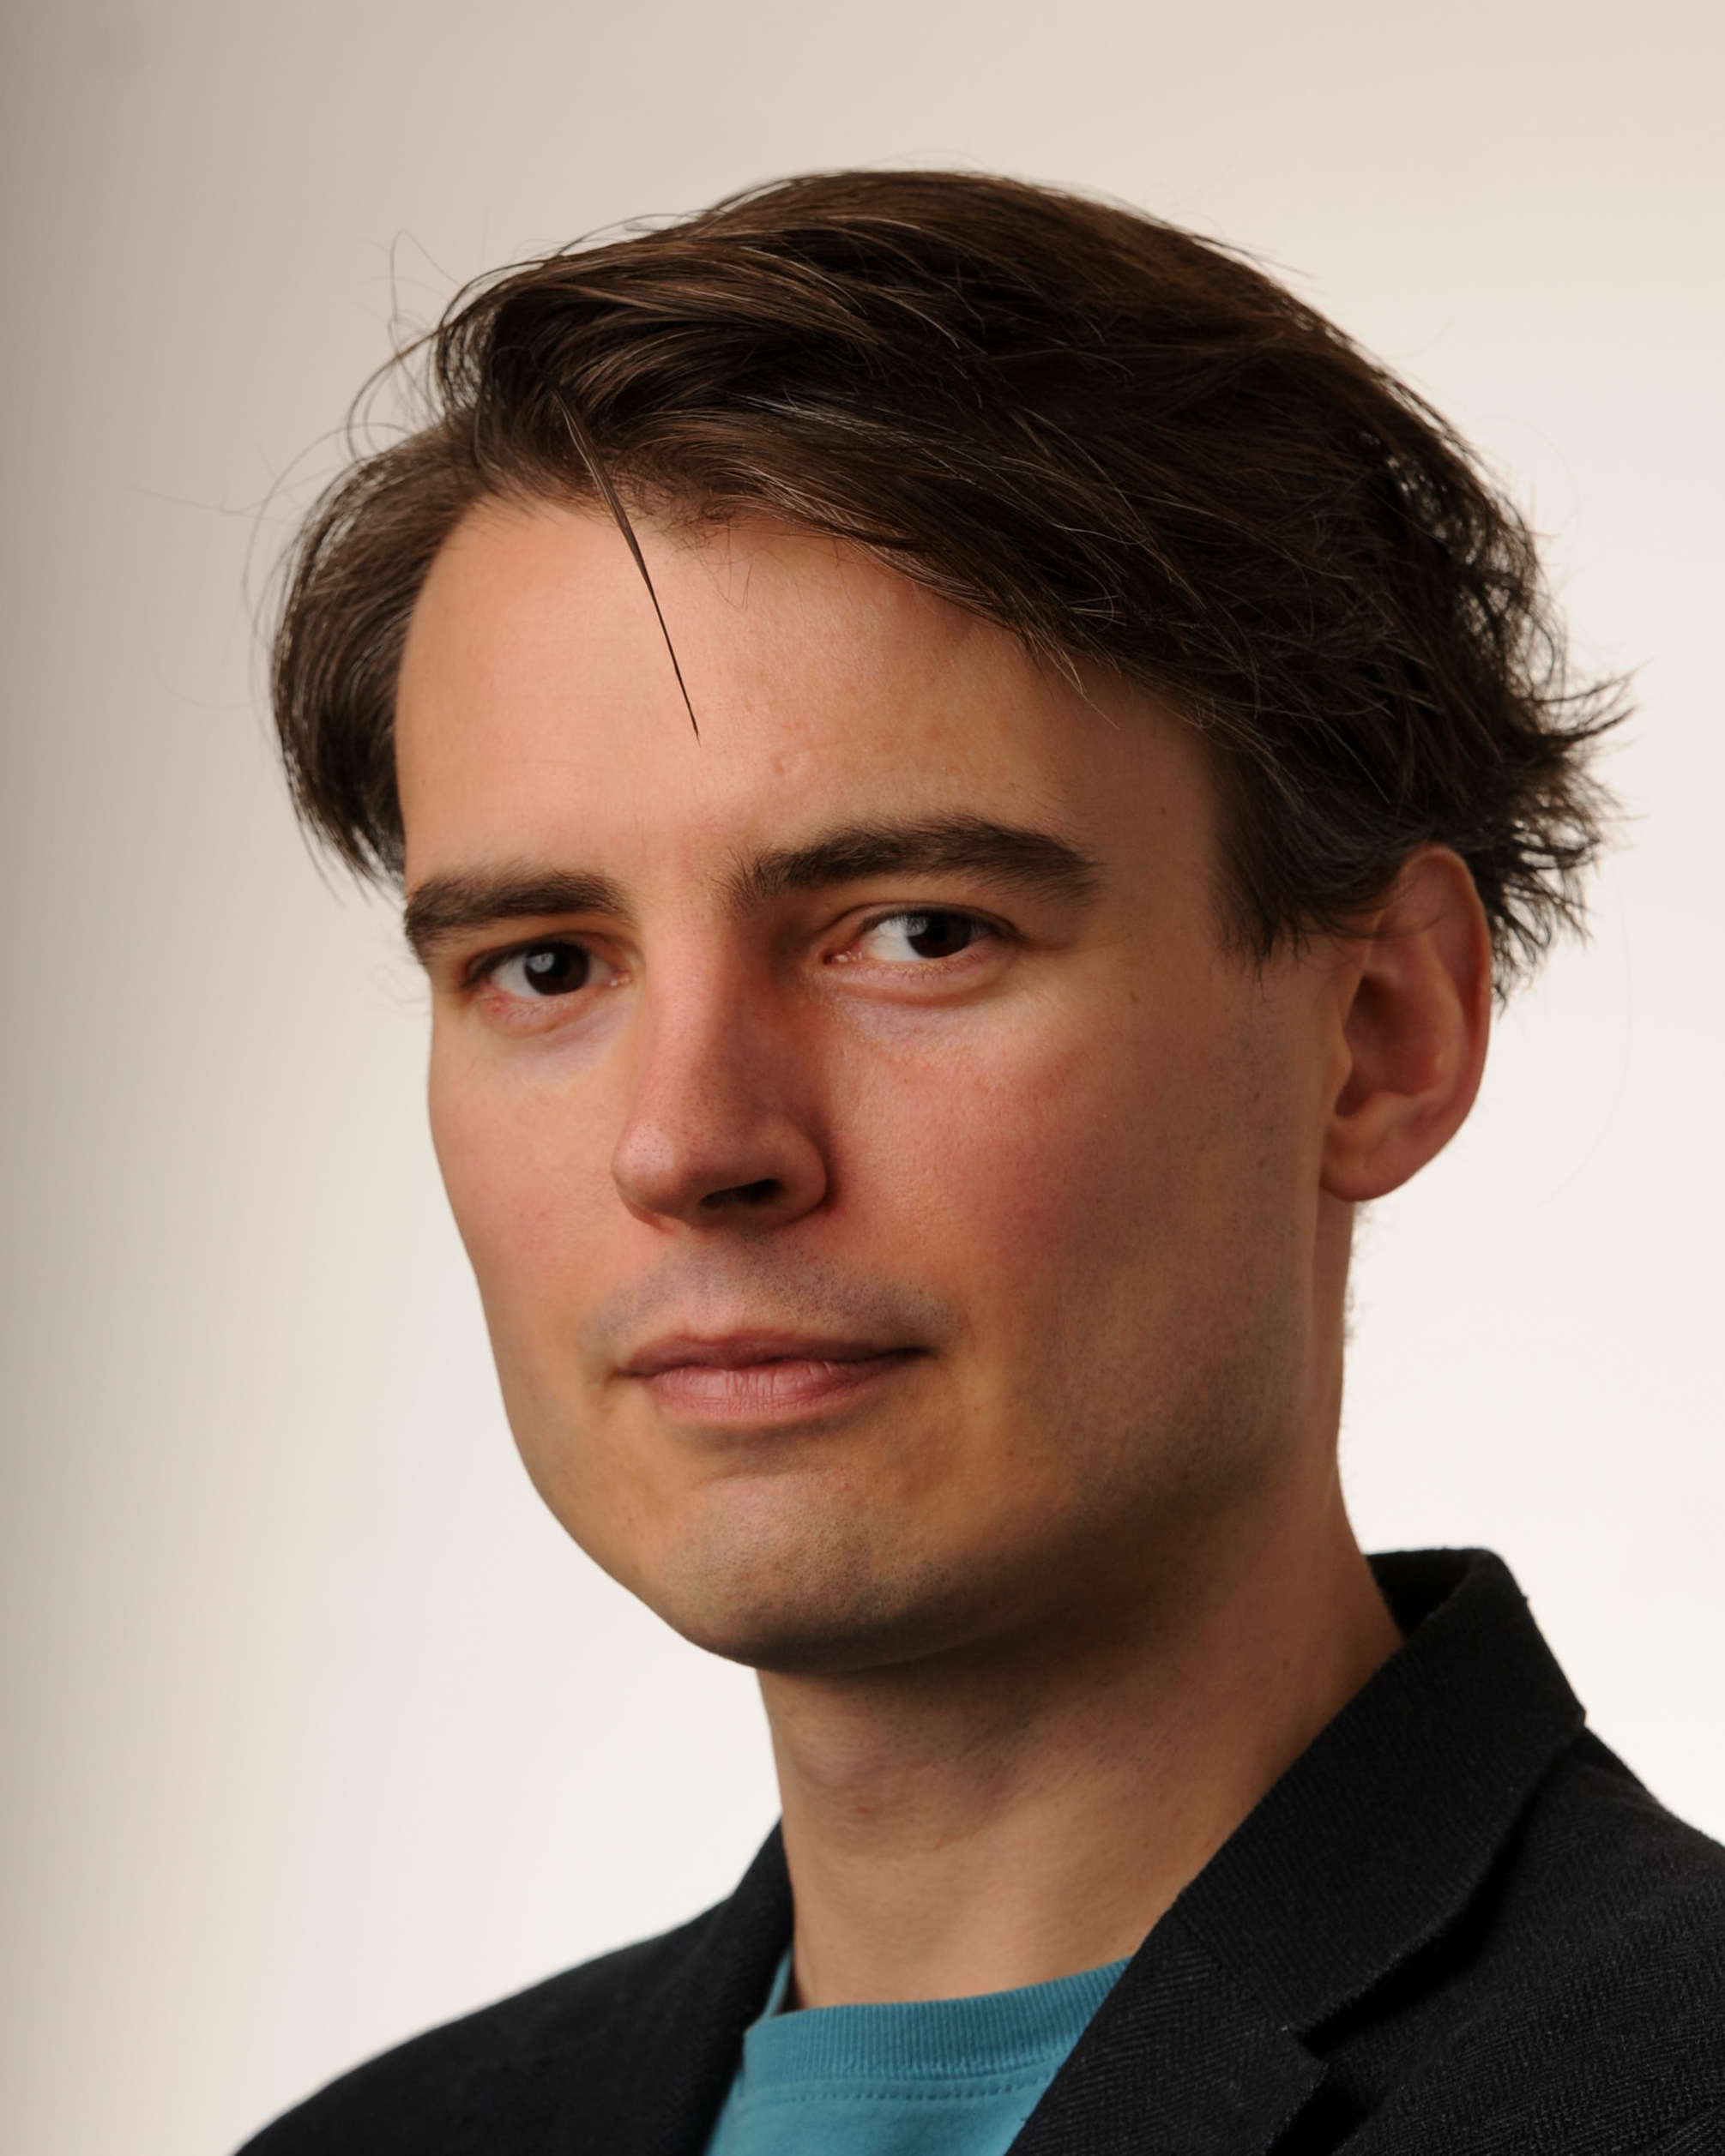
\includegraphics[width=4.5cm]{introduction/images/holger_pirk.jpg}};
		\end{tikzpicture}
		\centerline{\textbf{Dr Holger Pirk}}
	\end{center}
	\textbf{First Half}
	\begin{itemize}
		\item Hardware efficiency in complex systems
		\item Scaling up
		\item \textit{"getting the most bang for buck"}
	\end{itemize}
}{
	\begin{center}
		\begin{tikzpicture}
			\clip (0,0)  circle (2cm) ;
			\node[anchor=center] at (-.1,0.0) {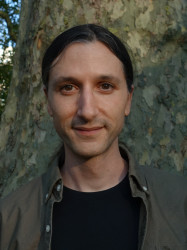
\includegraphics[width=4.5cm]{introduction/images/luis_vilanova.jpg}};
		\end{tikzpicture}
		\centerline{\textbf{Dr Luis Vilanova}}
	\end{center}
	\textbf{Second Half}
	\begin{itemize}
		\item Scale out Processing
	\end{itemize}
}

\subsection{Extra Resources}
\unfinished

\section{What is System Performance Engineering}
\begin{definitionbox}{System}
    A collection of components interacting to achieve a greater goal.
    \begin{itemize}
        \item Usually applicable to many domains (e.g a database, operating system, webserver). The goal is domain-agnostic
        \item Designed to be flexible at runtime (deal with other interacting systems, real conditions) (e.g OS with user input, database with varying query volume and type)
        \item Operating conditions are unknown at development time (Database does not know schema prior, OS does not know number of users prior, Tensorflow does not know matrix dimensionality prior)
    \end{itemize}
    Large \& complex systems are typically developed over years by multiple teams.
\end{definitionbox}

The challenge with \textit{system performance engineering} is to make systems maintainable, widely applicable and fast.
\begin{center}
    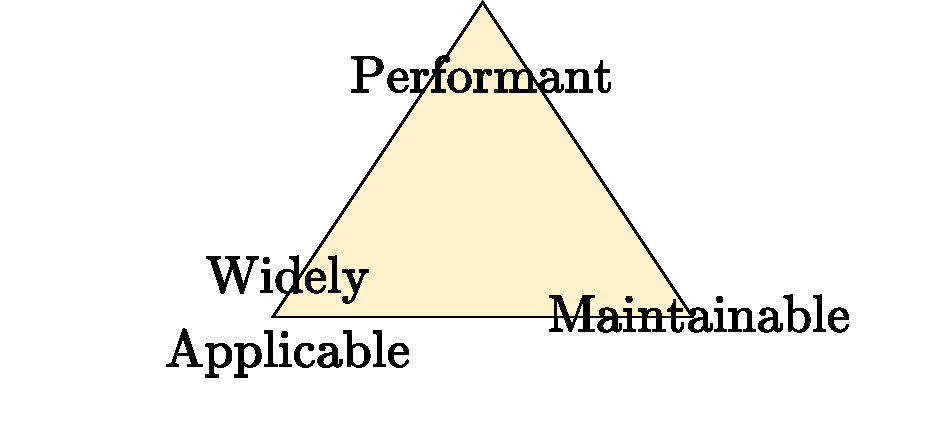
\includegraphics[width=.6\textwidth]{introduction/images/holy_triangle.drawio}
\end{center} 

\begin{definitionbox}{System Performance Engineering}
    Performance engineering encompasses the techniques applied during a systems development life cycle to ensure the non-functional
    requirements for performance will be met.
    \begin{itemize}
        \item Functional requirements (correctness, features) are assumed to be met.
        \item 
    \end{itemize} 
\end{definitionbox}

\begin{definitionbox}{High Performance Computing}
    High performance programming uses highly distributed \& parallel computer systems (e.g supercomputers, clusters) to solve advanced problems.
    \begin{itemize}
        \item Focuses on solving a single computationally difficult problem.
        \item Workloads are well defined and known at development time.
        \item Sometimes supported by custom hardware (e.g FPGAs, ASICs, custom CPU extensions)
    \end{itemize}
\end{definitionbox}

\section{Performance Engineering Process}
\subsection{Metrics}
A \textit{target metric} is used to quantitatively measure any improvement in \textit{performance} (e.g for use in a \textit{SLA}).
The metric needs to be wel defined:
\begin{itemize}
    \item When measuring starts (e.g when to measure latency from)
    \item Where measuring is done (is server response time measured on server, on a client, under what conditions?)    
\end{itemize}

\begin{examplebox}{Imperials}
    Provide some example of metrics regarding a database.
    \tcblower
    \begin{center}
        \begin{tabular}{l p{.7\textwidth}}
            \textbf{Latency} & Measuring time to query, planning time, the whole systems response time over a network. \\
            \textbf{Throughput} & Measure the maximum request/second possible (often used to compare webservers) \\
            \textbf{Memory Usage} & measurable, but must be careful (e.g os interaction) \\
            \textbf{Scalability} & Can define a metric regarding how quickly some metric (e.g throughput) increases with scale (e.g instances of a distributed system) \\
        \end{tabular}
    \end{center}
\end{examplebox}    

It is also important to define when a requirement is satisfied.
\begin{itemize}
    \item Setting an optimisation budget (e.g in developer hours)
    \item Setting a target or threshold (e.g $x\%$ over baseline implementation)
    \item Combination of both
\end{itemize}

\subsection{Quality of Service (QoS) Objectives}
\begin{definitionbox}{Quality of Service Objectives}
    A set of statistical properties of a metric that must hold for a system.
    \begin{itemize}
        \item Can include preconditions (e.g to define the environment/setup)
        \item Can be in conflict with functional requirements (e.g framerate vs realism in graphics)
    \end{itemize}
\end{definitionbox}
\begin{examplebox}{Game On}
    Give an example of a basic QoS Objective for a game's framerate. 
    \tcblower
    The game's framerate will be on average (over \textit{\dots preconditions \dots}) $60fps$ if run on a GPU rated at $50GFlops$ or higher. 
\end{examplebox}

\subsection{Service Level Agreements}
\begin{definitionbox}{Service Level Agreements (SLAs)}
    Legal contracts specifying \textit{QoS objectives} and penalties for violation.
    \begin{itemize}
        \item Non-functional requirements (not about system correctness)
        \item Can be legally enforced
    \end{itemize}
\end{definitionbox}

\begin{sidenotebox}{Amazon}
    Amazon Web Services (AWS) provides a set of \textit{service level agreements} relating to performance and availability. Violations are resolved by providing customers with service credits.
    \href{https://aws.amazon.com/compute/sla/}{Amazon SLAs}
\end{sidenotebox}

When defining requirements for an SLA:
\begin{center}
    \begin{tabular}{l p{.7\textwidth}}
        \textbf{Specific} & State exact acceptance criteria (numerical terms). \\
        \textbf{Measurable} & Ensure the metrics used can actually be measured. \\
        \textbf{Acceptable} & Requirements should be rigorous such that meeting them is a meaningful success. \\
        \textbf{Realisable} & Counter to \textbf{Acceptable} - need to be lenient enough to allow implementation. \\
        \textbf{Thorough} & All necessary aspects of the system are specified. \\
    \end{tabular}
\end{center}

\section{Performance Evaluation Techniques}
\subsection{Measuring}
\begin{itemize}
    \item Performed on the actual system (can be prototype or production/final).
    \item Can be difficult and costly (need to mitigate any impact of the measuring system on the system itself).
    \item As it is on the actual system, it can (if done properly) yield accurate results.
\end{itemize}

The two main types of measurement are:
\begin{tcbraster}[raster columns=2,raster equal height]
\begin{definitionbox}{Monitoring}
    Measuring in production to get real usage performance metrics.
    \begin{itemize}
        \item Observe the system in its production environment
        \item Collect usage statistics and analyse data (e.g user's preferred query types/structure, schema designs for databases)
        \item Can monitor for and report SLA violations.
    \end{itemize}
\end{definitionbox}
\begin{definitionbox}{Benchmarking}
    Measuring system performance in a controlled setting (e.g lab).
    \begin{itemize}
        \item The system to set into a predefined (or steady/hot) state
        \item Perform some workload while measuring performance metrics.
    \end{itemize}
\end{definitionbox}
\end{tcbraster}
Benchmarking requires representative workloads in order to get metrics likely to be representative of a production environment.
\begin{definitionbox}{Batch Workload}
    Program has access to entire batch at start of the benchmark.
    \begin{itemize}
        \item Useful when a throughput metric is being measured
        \item Simple to generate, and can even be recorded from a production environment.
    \end{itemize}
\end{definitionbox}
\begin{definitionbox}{Interactive Workload}
    A program generates requests to pass to the system being benchmarked.
    \begin{itemize}
        \item Useful when a latency metric is being measured.
        \item Workload generator needs to fast enough to saturate system being benchmarked.
        \item Often more representative of a production environment (e.g an operating system receives a workload over time)
    \end{itemize}
\end{definitionbox}
\begin{definitionbox}{Hybrid}
    A common setup combining batch and interactive workload strategies (e.g sample random queries from a predefined work set).
\end{definitionbox}

In order to get useful results from which 

\section{Optimisation Loop}
\begin{center}
    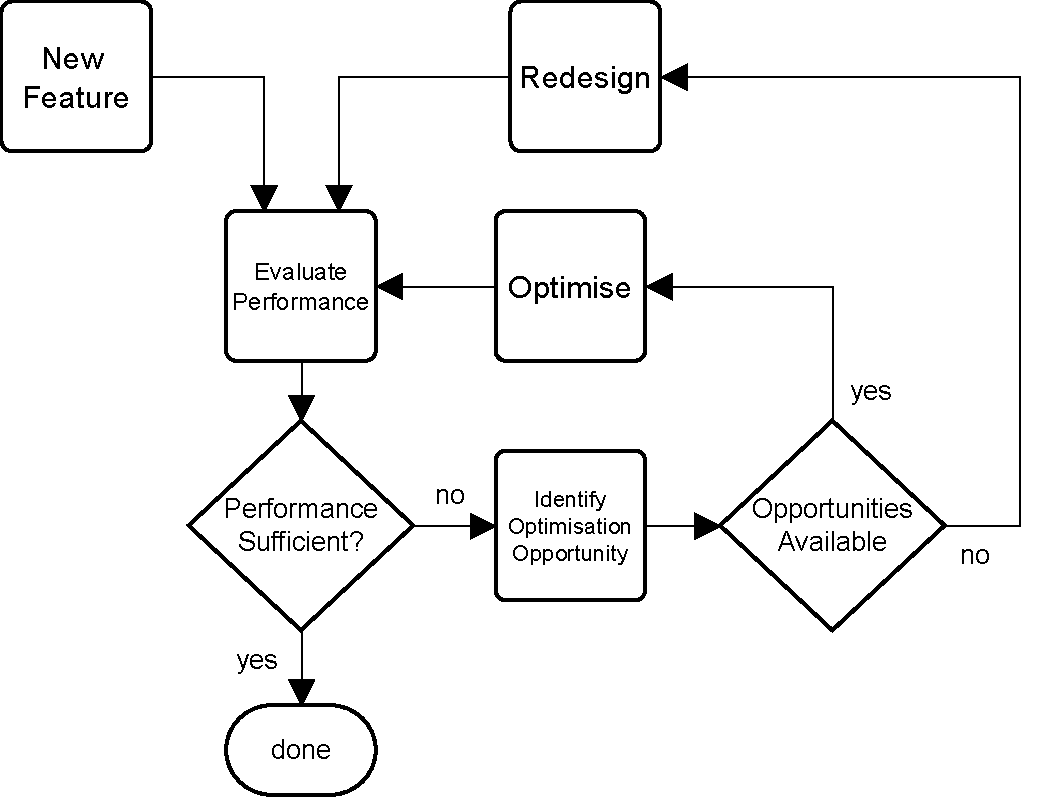
\includegraphics[width=.6\textwidth]{introduction/images/optimisation_loop.drawio.pdf}
\end{center}

\begin{definitionbox}{Performance Parameters}
    System and workload characteristics that affect performance.
     \\
     \\ \begin{tabular}{l p{.8\textwidth}}
        \textbf{System Parameters} & Do not change as the system runs (instruction costs, caches) \\
        \textbf{Workload Parameters} & Change as he system runs (available memory, users) \\
        \textbf{Numeric Parameters} & Quantitative (e.g CPU frequency, available memory, number of user) \\
        \textbf{Nominal Parameters} & Qualitative parameters (Runs on battery, has a GPU, runs in a VM) \\
    \end{tabular}
    \\ 
    \\ The term \textit{resource Parameters/Resources} refers to the parameters of the underlying platform (e.g CPU, memory).
\end{definitionbox}


\begin{tcbraster}[raster columns=2,raster equal height]
\begin{definitionbox}{Utilisation}
    The proportion of a resource used by a to perform a service by a system.
    \begin{itemize}
        \item A service has limited resources available (e.g CPU time, memory capacity, network bandwidth etc)
        \item Total available resources/resource budget available to a service is a parameter
    \end{itemize}
\end{definitionbox}
\begin{definitionbox}{Bottleneck}
    The resource with the highest utilisation.
    \begin{itemize}
        \item The limiting factor in performance of a system
        \item given some resource $x$ is the bottleneck, the system is $x$-bound (e.g CPU-bound). 
        \item Not always a resource, and performance may be bottlenecked by some other factor (e.g latency-bound $\to$ the system is dominated by waiting for some operation)
    \end{itemize}
\end{definitionbox}
\end{tcbraster}
It is typically infeasible to identify all bottlenecks for an entire complex software system.

To limit optimisation complexity efforts should be restricted to optimising code paths that have particularly large effect on performance.
\begin{tcbraster}[raster columns=2,raster equal height]
    \begin{definitionbox}{Critical Path}
        The sequence of activities which contribute the larges overall duration.
    \end{definitionbox}
    \begin{definitionbox}{Hot Path}
        A code path where most of the execution time is spent (e.g very commonly executed subroutine)
    \end{definitionbox}
\end{tcbraster}

In order to optimise we require:
\begin{itemize}
    \item Ability to quickly compare alternative designs
    \item Ability to select a near optimal value for platform parameters
\end{itemize}
While workload parameters are not typically controllable at this stage, some system parameters are.

\begin{definitionbox}{Parameter Tuning}
    Finding the vector within the parameter space that minimises resource usage, or maximises performance.
    \begin{itemize}
        \item Exploring the parameter space is expensive (even with non-linear optimisation)
        \item Analytical models can be used to accelerate search.
        \item Tuning needs to consider tradeoffs (e.g much of a cheap resource versus little of an expensive one)
    \end{itemize}
\end{definitionbox}

\begin{definitionbox}{Analytical Performance Model}
    A model describing the relationship between system parameters and performance metrics.
    \begin{itemize}
        \item Having an accurate analytical model for the system is analogous to \textit{understanding} the performance of the system.
        \item Models can be stateless (e.g an equation) or stateful (e.g using markov chains).
        \item Need to model dynamic systems with (ideally small) static models.
        \item Very fast (faster than search parameter space)
        \item Allow for \textit{what-if analysis} of system and workload parameters.
    \end{itemize}
\end{definitionbox}

\begin{definitionbox}{Simulation}
    A single observed run of a stateful model
    \begin{itemize}
        \item Can see all interactions within the system in perfect detail
        \item Extremely expensive to run (limiting number of simulations and the speed of the optimisation workflow)
        \item Much more rarely used than other techniques described
    \end{itemize}
\end{definitionbox}

